\documentclass[10pt]{beamer}

\usefonttheme{professionalfonts}% use own font handling
% \usetheme{m}

\usepackage{ulem}
\usepackage{turnstile}
\usepackage{proof}
\usepackage{booktabs}
\usepackage[scale=2]{ccicons}
\usepackage{amsmath, stmaryrd, scalerel}
\usepackage{fontspec}
\usepackage{geometry}
\usepackage{proof}
\usepackage{supertabular}
\usepackage{unicode-math}
\usepackage{xltxtra}
\usepackage{xunicode}
\setmathfont{Asana Math}

% \theoremstyle{mystyle}
\newtheorem*{remark}{Remark}

% colors
\definecolor{MidnightBlue}{rgb}{0.1, 0.1, 0.44}
\definecolor{Maroon}{rgb}{0.5, 0.0, 0.0}
\def\InputModeColorName{MidnightBlue}
\def\OutputModeColorName{Maroon}

% modes
\newcommand\IMode[1]{{\color{\InputModeColorName}{#1}}}
\newcommand\OMode[1]{{\color{\OutputModeColorName}{#1}}}

\newcommand\Member[2]{\IMode{#1}\in \IMode{#2}}
\newcommand\Nat{\mathbb{N}}

\title{Won't you bar my neighbor[hood]?}
\subtitle{brouwer's realizability and the bar principle}
\date{\today}
\institute{SlamData, Inc.}
\author{Jon Sterling}

\begin{document}

\maketitle

\section{Introduction}

\begin{frame}
  \frametitle{Spreads as Spaces and Trees}
  \pause
  A \emph{spread} is at the same time a \alert{topological space} and a \alert{non-wellfounded tree}.

  \medskip

  \pause
  A spread is defined by a predicate $\mathfrak{S}$ on lists of natural numbers subject to some laws:
  \pause
  \begin{enumerate}
    \item If $\Member{\vec{u}}{\mathfrak{S}}$, then there exists an $\Member{x}{\Nat}$ such
      that $\Member{\vec{u}\frown x}{\mathfrak{S}}$.
      \pause
    \item If $\Member{\vec{u}\frown x}{\mathfrak{S}}$, then also $\Member{\vec{u}}{\mathfrak{S}}$.
      \pause
    \item Finally, $\Member{[]}{\mathfrak{S}}$.
  \end{enumerate}

  \medskip
  \pause
  The predicate $\mathfrak{S}$ either defines the finite prefixes of paths down
  an infinite tree, or it defines the lattice of open sets of a topological space.

  \medskip
  \pause

  \alert{Usually, we will work implicitly with the \emph{universal spread}, which always says ``yes''.}

\end{frame}

\begin{frame}
  \frametitle{Neighborhoods and Points, Prefixes and Paths}

  A list of naturals $\Member{\vec{u}}{\Nat*}$ can be thought of as a \alert{neighborhood} around a point, or as a \alert{prefix} of a path through an infinite tree.
  \medskip

  \pause

  A stream of naturals $\Member{\alpha}{\Nat^\Nat}$ can be thought of as an \alert{ideal point} in the spread (space), or as a \alert{path} through the spread's infinite tree.

  \pause

  \begin{align*}
    \IMode{\vec{u}}\prec\IMode{\alpha}
    \tag{$\IMode{\vec{u}}$ approximates $\IMode{\alpha}$}\\
    \Member{\alpha}{\vec{u}}
    \tag{$\IMode{\vec{u}}$ is a neighborhood around $\IMode{\alpha}$}
  \end{align*}
\end{frame}

\begin{frame}
  \frametitle{Spread Visualization}
  \begin{figure}
  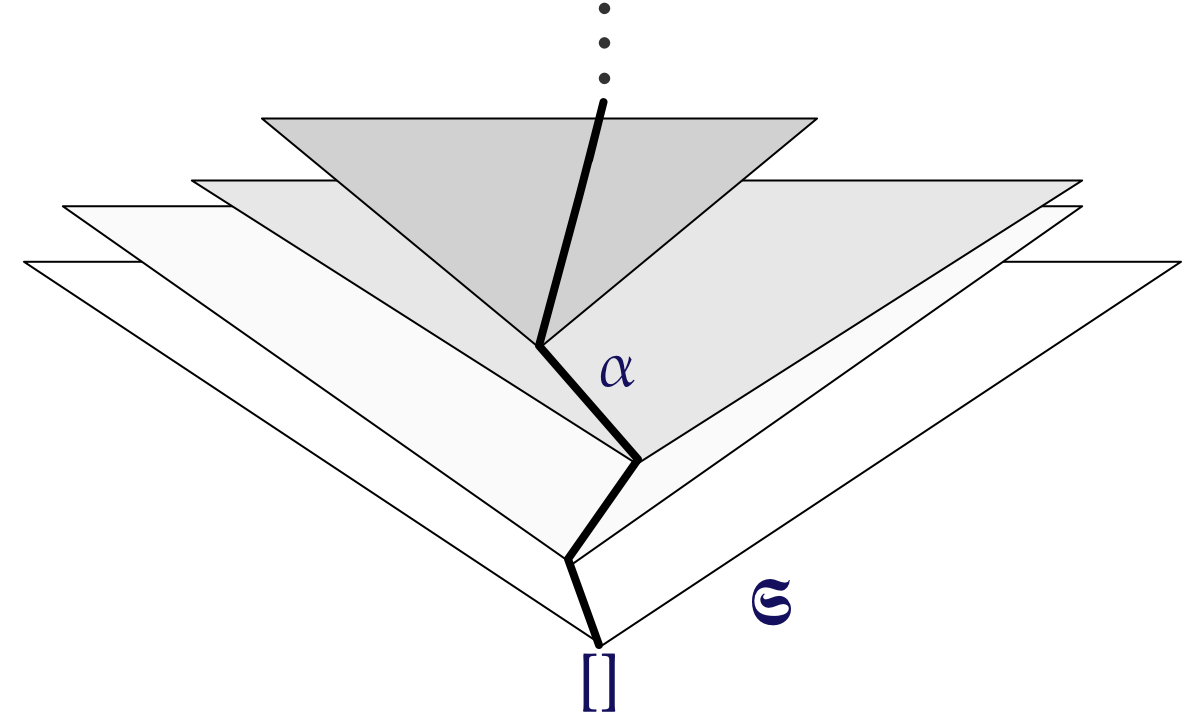
\includegraphics[width=0.9\linewidth]{illustrations/spread.png}
  \end{figure}
\end{frame}

\begin{frame}
  \frametitle{Bars and Securability}

  A \alert{bar} $\mathfrak{B}$ is a predicate on neighborhoods such that every
  point ``hits it''.  More generally, $\mathfrak{B}$ \alert{bars} a
  neighborhood $\vec{u}$ when every path through $\vec{u}$ ends up in $\mathfrak{B}$.

  \pause
  \[
    \forall \Member{\alpha}{\vec{u}}.\
    \exists \Member{\vec{v}}{\mathfrak{B}}.\
    \Member{\alpha}{\vec{v}}
  \]
  \begin{center}or equivalently\end{center}
  \[
    \forall \Member{\alpha}{\vec{u}}.\
    \exists \Member{n}{\Nat}.\
    \Member{\bar{\alpha}[n]}{\mathfrak{B}}
  \]

  \pause

  We say that a neighborhood is \alert{secured} when it is in the bar, and that
  it is \alert{securable} when every path out of it eventually hits the bar.
\end{frame}

\begin{frame}
  \frametitle{Visualizing Bars}
  \only<1>{
    \begin{figure}
    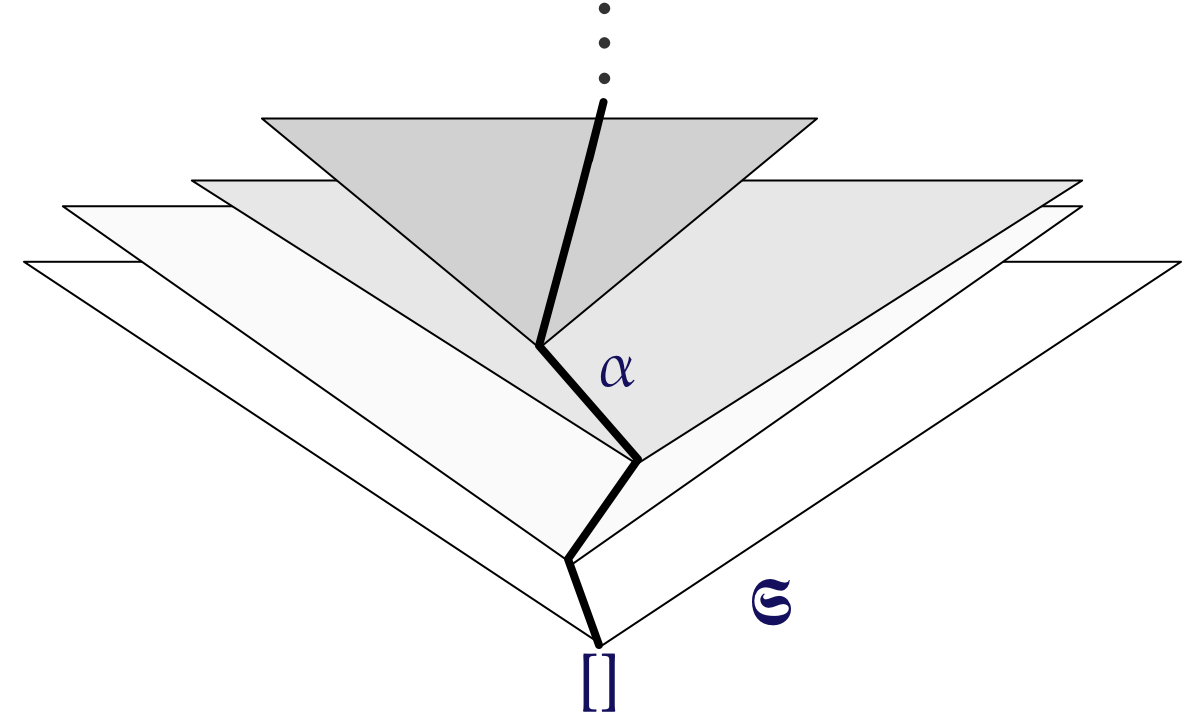
\includegraphics[width=0.9\linewidth]{illustrations/spread.png}
    \end{figure}
  }
  \only<2>{
    \begin{figure}
    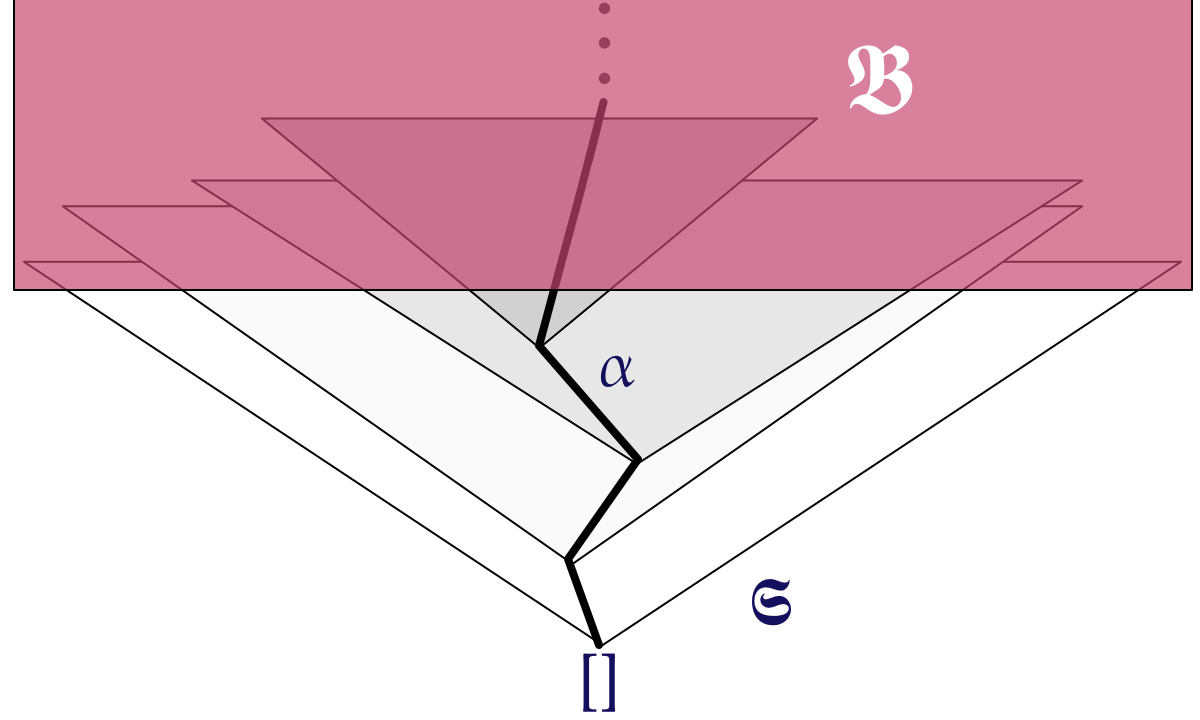
\includegraphics[width=0.9\linewidth]{illustrations/spread-with-bar.png}
    \end{figure}
  }
\end{frame}

\begin{frame}
  \begin{itemize}
    \item bars represent inevitability
      \pause
    \item bars represent termination
      \pause
    \item \alert{bars let us reason by induction on infinite trees}
  \end{itemize}
  \pause
  \begin{center}
    (intuitionistic and classical, not constructive)
  \end{center}
\end{frame}

\begin{frame}
  \frametitle{The Bar Induction Principle}

  Let $\mathfrak{B}$ be a \alert{decidable bar}; let $\mathfrak{A}$ be another
  predicate on neighborhoods (the \alert{motive} of induction). Suppose:
  \pause

  \begin{enumerate}
    \item Every $\mathfrak{B}$-\alert{secured} neighborhood is also in $\mathfrak{A}$.
      \[
        \forall\Member{\vec{u}}{\mathfrak{B}}.\
        \Member{\vec{u}}{\mathfrak{A}}
      \]
      \pause
    \item If every immediate refinement of a neighborhood is in $\mathfrak{A}$, then that neighborhood is also in $\mathfrak{A}$.
      \[
        \forall\Member{\vec{u}}{\mathfrak{A}}.\
        \left(\forall\IMode{x}.\Member{\vec{u}\frown x}{\mathfrak{A}}\right)
        \Rightarrow
        \Member{\vec{u}}{\mathfrak{A}}
      \]
  \end{enumerate}

  \pause
  Then, every $\mathfrak{B}$-\alert{securable} neighborhood is also in $\mathfrak{A}$.
  Or, equivalently:
  \[
    \Member{[]}{\mathfrak{A}}
  \]
\end{frame}

\begin{frame}
  \frametitle{What is the constructive meaning of the bar principle?}

  It asserts that the \alert{evidence} that $\vec{u}$ is
  $\mathfrak{B}$-securable is a wellfounded/inductive tree.

  \medskip
  \pause

  Then, clause (1) gives us the \alert{base case}, and clause (2) gives us the
  \alert{inductive step} for concluding $\Member{\vec{u}}{\mathfrak{A}}$.

  \medskip
  \pause

  The proof of $\Member{\vec{u}}{\mathfrak{A}}$ proceeds by considering the possible ways in which $\vec{u}$ could be $\mathfrak{B}$-securable:
  \begin{itemize}
    \item[$\eta\;\blacktriangleright$]
      $\vec{u}$ is $\mathfrak{B}$-secured.
    \item[$\zeta\;\blacktriangleright$]
      $\IMode{\vec{u}}\equiv\OMode{\vec{v}\frown x}$ such that $\vec{v}$ is $\mathfrak{B}$-securable
    \item[$\digamma\;\blacktriangleright$]
      For all immediate refinements $x$, $\vec{u}\frown x$ is $\mathfrak{B}$-securable
  \end{itemize}

\end{frame}
\begin{frame}
  \frametitle{Normalizing securability}

  We have identified three different ways that $\vec{u}$ could be $\mathfrak{B}$-securable:
  \medskip

  \begin{itemize}
    \item[$\eta\;\blacktriangleright$]
      $\vec{u}$ is $\mathfrak{B}$-secured.
    \item[$\zeta\;\blacktriangleright$]
      $\IMode{\vec{u}}\equiv\OMode{\vec{v}\frown x}$ such that $\vec{v}$ is $\mathfrak{B}$-securable
    \item[$\digamma\;\blacktriangleright$]
      For all immediate refinements $x$, $\vec{u}\frown x$ is $\mathfrak{B}$-securable
  \end{itemize}

  \medskip
  \pause

  \alert{In fact, we can always normalize a proof built from these primitives into one
  which contains only $\eta$ and $\digamma$ inferences.}

  \medskip
  \pause

  Then, every $\eta$-inference is replaced with the \alert{base case}, and
  every $\digamma$-inference is replaced with the \alert{inductive step}, obtaining
  a proof that $\Member{\vec{u}}{\mathfrak{A}}$.
\end{frame}

\begin{frame}
  \frametitle{So what's the problem?}
  \pause

  The inductive characterization of bar-hood in terms of $\eta,\zeta,\digamma$
  is not necessarily the same as the formal/logical definition:
  \[
    \forall \Member{\alpha}{\vec{u}}.\
    \exists \Member{n}{\Nat}.\
    \Member{\bar{\alpha}[n]}{\mathfrak{B}}
  \]

  \medskip
  \pause

  In fact, if we interpret this statement using \alert{propositions-as-types},
  then it is \alert{not the same}! There is a procedure to convert a program
  realizing this statement into a well-founded $\eta,\zeta,\digamma$-tree, but
  to show that this procedure terminates, we need the bar induction principle
  already in the metatheory.

  \medskip
  \pause
  \alert{So, what would Brouwer say to this?}

\end{frame}

\begin{frame}
  \frametitle{Brouwerian Realizability: Neighborhood Functions}

  A point in the spread is an infinite stream of natural numbers. For Brouwer,
  a function that processes a stream is \alert{not} a function from streams to results.

  \[
    \mathsf{stream}(\Nat) \to X
    \tag{\alert{not this!}}
  \]

  \medskip
  \pause

  Rather, it is a \alert{neighborhood function}, a monotonic \& continuous
  function from \alert{neighborhoods} to \alert{partial results}:

  \pause

  \[
    \left\{
      \Member{\phi}{\Nat*\to (\mathbb{1}\oplus X)}
      \mid P(\IMode{\phi})
    \right\}
  \]
  \[
    P(\IMode{\phi}) \equiv
      \forall\Member{\alpha}{\mathsf{stream}(\Nat)}.\
      \exists\Member{k}{\Nat}.\
      \exists\Member{a}{X}.\
      \forall\IMode{k'}\geq\IMode{k}.\
      \IMode{\phi\left(\bar{\alpha}[k']\right)}\equiv\IMode{\mathsf{inr}(a)}
  \]
\end{frame}

\begin{frame}
  \frametitle{Well-Ordering Neighborhood Functions}
  \[
    \left\{
      \Member{\phi}{\Nat*\to (\mathbb{1}\oplus X)}
      \mid P(\IMode{\phi})
    \right\}
  \]
  \[
    P(\IMode{\phi}) \equiv
      \forall\Member{\alpha}{\mathsf{stream}(\Nat)}.\
      \exists\Member{k}{\Nat}.\
      \exists\Member{a}{X}.\
      \forall\IMode{k'}\geq\IMode{k}.\
      \IMode{\phi\left(\bar{\alpha}[k']\right)}\equiv\IMode{\mathsf{inr}(a)}
  \]

  The condition $P$ on a neighborhood function $\phi$ induces a well-ordering
  on $\phi$'s graph. That is, each such function can be identified with some well-founded
  \alert{dialogue tree}.
\end{frame}

\begin{frame}
  \frametitle{Neighborhood Functions for Securability}

  ``$\vec{u}$ is $\mathfrak{B}$-securable'':
  \[
    \forall \Member{\alpha}{\vec{u}}.\
    \exists \Member{n}{\Nat}.\
    \Member{\bar{\alpha}[n]}{\mathfrak{B}}
  \]

  \medskip
  \pause

  As far as Brouwer is concerned, the evidence for this statement is a
  dependent \alert{neighborhood function}:
  \[
    \prod_{\IMode{\vec{v}}\succcurlyeq\IMode{\vec{u}}}
    \mathbb{1}
    \oplus
    \sum_{\Member{n}{\Nat}}
    \Member{\vec{v}[\vert\vec{u}\vert + n]}{\mathfrak{B}}
  \]

  By the same technique mentioned before, we can identify any such function
  with a wellfounded tree.
\end{frame}

\begin{frame}
  \frametitle{Neighborhood Functions for Securability}
  \[
    \prod_{\IMode{\vec{v}}\succcurlyeq\IMode{\vec{u}}}
    \mathbb{1}
    \oplus
    \sum_{\Member{n}{\Nat}}
    \Member{\vec{v}[\vert\vec{u}\vert + n]}{\mathfrak{B}}
  \]

  By the same technique mentioned before, we can identify any such function
  with a wellfounded tree, in particular a $\eta,\zeta,\digamma$-tree.
  \pause

  \begin{itemize}
    \item $\IMode{\mathsf{inl}(*)}$ corresponds to a $\OMode{\digamma}$-inference
      \pause

    \item $\IMode{\mathsf{inr}(0,\mathcal{D})}$ corresponds to an $\OMode{\eta}$-inference
      \pause
    \item $\IMode{\mathsf{inr}(n+1,\mathcal{D})}$ corresponds to an $\OMode{\zeta}$-inference
  \end{itemize}

  \medskip
  \pause

  \alert{%
    \emph{%
      Therefore, the Bar Principle is true under a Brouwerian explanation of the
      logical connectives!
    }
  }
\end{frame}

\begin{frame}
  \frametitle{Status of BI in Type Theory}
  \pause

  \begin{itemize}
    \item
      There are models of type theory that refute the Bar Principle:
      \alert{recursive realizability} (via Church's Thesis), etc.

      \pause
    \item
      The Bar Principle relies on an \alert{open-ended notion of stream}, i.e.\ one which does
      not require that all streams be computed by a recursive function.

      \pause
    \item
      Adding the Bar Principle to Type Theory is harmless, but \alert{restricts the
      possible models}.
\end{itemize}

\end{frame}

\begin{frame}
  \frametitle{Concluding Thoughts}

  To add the Bar Principle as an axiom to Type Theory is to formalize our intention that
  Type Theory shall be a semi-formal theory of constructions for Brouwer's mathematics.
\end{frame}

% \nocite{*}
% \begin{frame}[allowframebreaks]
%
%   \frametitle{References}
%
%   \bibliography{refs}
%   \bibliographystyle{abbrv}
%
% \end{frame}

\end{document}
